\subsection{The Radical of a Ring}

DEFINITION 2. --- The Jacobson radical (or simply radical) of a ring A, denoted by \(\Re(\mathrm{A})\) , is the radical of the A-module \(A_{s}\) , that is, the intersection of the maximal left ideals of A.

By abuse of language, we say that the ring A is without radical if we have \(\Re(A)=0\) .

PROPOSITION 4. --- A ring A is semisimple if and only if it is left Artinian and without radical.

This follows from Proposition 3, b) applied to the A-module \(\mathrm{A}_s\) .

Examples. --- 1) If A is a local ring, then it has a unique maximal left ideal r, consisting of the noninvertible elements of A (VIII, p.~25, Proposition 1); so r is the radical of A. In particular, a field is without radical.

\pandocbounded{
\includegraphics[keepaspectratio]{images/part001_b3b59696.jpg}}

\begin{enumerate}
\def\labelenumi{\arabic{enumi})}
\setcounter{enumi}{1}
\item
  Let K be a commutative field and E the algebra \(\mathrm{K}[[\mathrm{X}_{i}]]_{i\in\mathrm{I}}\) of formal power series in the variables \(X_{i}\) with coefficients in K. By the previous example and Example 4 of VIII, p.~26, the radical of E consists of the formal power series with constant term zero. Observe that the ring E is an integral domain and that its radical is not reduced to 0, even though E is a subring of its field of fractions, which is without radical.
\item
  Suppose that A is a principal ideal domain, and let P be a system of representatives consisting of irreducible elements (VII, §1, No.~3, p.~3). If A is a field, then it is without radical by Example 1. If the set P is infinite, then the intersection of the maximal ideals Ap of A is reduced to 0, so A is without radical. But if P is finite and nonempty, and if we set \(x = \prod_{p \in P} p\) , then the radical of A is equal to \(\cap_{p \in P} Ap = Ax\) (VII, §1, No.~2, p.~3, Proposition 4), hence is not reduced to 0.
\end{enumerate}

Let y be a nonzero element of A; we write it as \(y = up_{1}^{i_{1}} \cdots p_{r}^{i_{r}}\) , where u is invertible in A, \(p_{1}, \ldots, p_{r}\) are pairwise distinct elements of P, and \(i_{1}, \ldots, i_{r}\) are strictly positive integers. The maximal ideals of the ring A/Ay are the ideals \(Ap_{1}/Ay, \ldots, Ap_{r}/Ay\) ; the radical of the ring A/Ay is therefore the ideal \(Ap_{1} \cdots p_{r}/Ay\) . In particular, the ring A/Ay is without radical if and only if we have \(i_{1} = \cdots = i_{r} = 1\) ; in this case, we say that y is without multiple factors.

PROPOSITION 5. --- a) The radical of a ring A is the intersection of the annihilators of simple A-modules; it is also the smallest annihilator of a semisimple A-module. It is, in particular, a two-sided ideal of A. If A is not reduced to 0, then the radical of A is distinct from A.

\begin{enumerate}
\def\labelenumi{\alph{enumi})}
\setcounter{enumi}{1}
\item
  Let \(\mathfrak{a}\) be a two-sided ideal of A. We have \((\Re (\mathrm{A}) + \mathfrak{a}) / \mathfrak{a} \subset \Re (\mathrm{A} / \mathfrak{a})\) . If \(\mathfrak{a}\) is contained in \(\Re (\mathrm{A})\) , then we have \(\Re (\mathrm{A} / \mathfrak{a}) = \Re (\mathrm{A}) / \mathfrak{a}\) .
\item
  The ring A/R(A) is without radical; conversely, every two-sided ideal a of A such that A/a is without radical contains R(A).
\item
  The radical of A is contained in the intersection of the maximal two-sided ideals of A.
\end{enumerate}

Let \(x \in \mathrm{A}\) . Saying that \(x\) belongs to the annihilator of every simple A-module is equivalent to saying that \(x\) belongs to the annihilator of every element of every simple A-module, in other words (VIII, p.~46, Proposition 1), to every maximal left ideal of A.

Let M be a semisimple A-module. Its annihilator is the intersection of the annihilators of the simple submodules of M, so it contains \(\Re(\mathrm{A})\) . Furthermore, if S is the set of classes of simple A-modules (VIII, p.~51), then the direct sum \(\oplus_{\lambda\in\mathcal{S}}\lambda\) is a semisimple A-module whose annihilator is \(\Re(\mathrm{A})\) . Suppose that A is not reduced to 0; the relation \(\Re(\mathrm{A})\neq\mathrm{A}\) follows from Proposition 2, a) of VIII, p.~153 applied to the A-module \(A_{s}\) . We have proved a).

Let \(\mathfrak{a}\) be a two-sided ideal of A. The maximal left ideals of A/ \(\mathfrak{a}\) are the ideals of the form \(\mathfrak{m}/\mathfrak{a}\) , where \(\mathfrak{m}\) is a maximal left ideal of A containing \(\mathfrak{a}\) . Consequently, the radical of the ring A/ \(\mathfrak{a}\) is equal to the radical of the A-module \(A_s/\mathfrak{a}\) . Assertions b) and c) therefore follow from Corollary 1 of VIII, p.~152.

Let \(\mathfrak{a}\) be a maximal two-sided ideal of A. In the ring A/ \(\mathfrak{a}\) , the only two-sided ideals are 0 and A/ \(\mathfrak{a}\) . Since the ring A/ \(\mathfrak{a}\) is not reduced to 0, its radical is not equal to A/ \(\mathfrak{a}\) . The ring A/ \(\mathfrak{a}\) is therefore without radical, and we have \(\Re(A) \subset \mathfrak{a}\) by c). This proves d).

We say that a left (or right) ideal of A is a nil ideal if it consists of nilpotent elements. We say that a two-sided ideal \(\mathfrak{a}\) of A is nilpotent if there exists an integer \(n \geqslant 1\) such that \(\mathfrak{a}^n = 0\) , that is (I, §8, No.~9, p.~107), such that we have \(x_1 \cdots x_n = 0\) for every sequence \((x_1, \ldots, x_n)\) of elements of \(\mathfrak{a}\) . Every nilpotent two-sided ideal is a nil ideal, but there can exist nil ideals that are not contained in a nilpotent two-sided ideal (VIII, p.~167, Exercise 9).

THEOREM 1 (Jacobson). --- The radical of a ring A consists of the elements \(x \in \mathbf{A}\) such that \(1 + ax\) is left invertible (I, §2, No.~3, p.~15) for every \(a \in \mathbf{A}\) . It is also the largest two-sided ideal \(\mathfrak{a}\) such that \(1 + x\) is invertible for every \(x \in \mathfrak{a}\) . The radical of \(\mathbf{A}\) contains every left nil ideal of \(\mathbf{A}\) .

The element 1 generates the A-module \(A_{s}\) , and \(1 + ax\) is left invertible if and only if it generates the A-module \(A_{s}\) . The first assertion of Theorem 1 is therefore a specific case of the corollary of Proposition 2 (VIII, p.~153).

Let \(x \in \Re(\mathrm{A})\) . By the above, \(1 + x\) is left invertible; let \(y\) be an element of \(\mathrm{A}\) such that \(y(1 + x) = 1\) . We then have \(1 - y = yx\) , so \(1 - y\) belongs to \(\Re(\mathrm{A})\) ; consequently, \(y\) is left invertible. Since \(y\) is also right invertible, it is invertible (I, §2, No.~3, p.~16, Proposition 3), and so is its right inverse \(1 + x\) .

Let a be a left ideal of A such that \(1 + x\) is invertible for every \(x \in a\) . This holds, for example, when a is a nil ideal because the relation \(x^{n} = 0\) implies that \(1 - x + \cdots + (-x)^{n-1}\) is the inverse of \(1 + x\) . Let \(x \in a\) . For every \(a \in A\) , we have \(ax \in a\) , so \(1 + ax\) is invertible; hence, we have \(x \in \Re(A)\) . It follows that a is contained in \(\Re(A)\) .

COROLLARY 1. --- The radical of A is equal to the radical of the opposite ring A°, that is, to the intersection of the maximal right ideals of A.

For every \(x \in \Re(A)\) , \(1 + x\) is invertible in the ring A, hence in the ring \(A^{\circ}\) . Since \(\Re(A)\) is a two-sided ideal of \(A^{\circ}\) , we have \(\Re(A) \subset \Re(A^{\circ})\) . The equality follows by interchanging the roles of A and \(A^{\circ}\) .

COROLLARY 2. --- An element of A is invertible if and only if its canonical image in the ring A/ \(\Re(A)\) is invertible.

The condition is obviously necessary. Let us prove that it is sufficient. Let x be an element of A whose canonical image in the ring \(\mathrm{A}/\Re(\mathrm{A})\) is invertible. There then exists an element y of A such that xy belongs to \(1 + \Re(\mathrm{A})\) . By Theorem 1, xy is invertible; hence x is right invertible. The proof that x is left invertible is analogous.

COROLLARY 3. --- The radical of the product of a family \((\mathrm{A}_{i})_{i\in\mathrm{I}}\) of rings is the product of the \(\mathfrak{R}(\mathrm{A}_{i})\) .

Let \(x = (x_{i})_{i\in \mathrm{I}}\) be an element of \(\prod_{i\in \mathrm{I}}\mathrm{A}_{i}\) . For every element \(a = (a_{i})_{i\in \mathrm{I}}\) of \(\prod_{i\in \mathrm{I}}\mathrm{A}_{i}\) , the element \(1 + ax\) is left invertible if and only if \(1 + a_{i}x_{i}\) is left invertible in \(\mathrm{A}_i\) for every \(i\in \mathrm{I}\) . Corollary 3 follows.

COROLLARY 4. --- The ring A is local if and only if the ring A/ \(\Re(A)\) is a field. If this is the case, then \(\Re(A)\) is the set of noninvertible elements of A.

Denote the set of noninvertible elements of A by r. If the ring A is local, then its radical is equal to r (VIII, p.~154, Example 1) and the ring A/r is a field (VIII, p.~26). Conversely, suppose that the ring A/R(A) is a field. By Corollary 2, we have \(\mathfrak{r} = \Re(\mathrm{A})\) , so r is a two-sided ideal of A. It follows that the ring A is local (VIII, p.~26, Definition 1).

Examples. --- 4) Let K be an integral domain, I a nonempty set, and A the polynomial ring \(K[X_{i}]_{i\in I}\) . Let us prove that the ring A is without radical. The only invertible elements of A are the invertible elements of K (IV, §1, No.~5, p.~9, Corollary 2). Let \(f \in \Re(A)\) . Choose an element \(i \in I\) . Then \(1 + fX_{i}\) is invertible (Theorem 1), which implies f = 0.

\pandocbounded{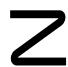
\includegraphics[keepaspectratio]{images/part001_fdd5464e.jpg}}

Note that when K is a commutative field, the ring \(A = K[X_{i}]_{i \in I}\) is a subring of \(B = K[[X_{i}]]_{i \in I}\) and we have \(\Re(A) = 0\) and \(A \cap \Re(B) \neq 0\) (cf.~VIII, p.~154, Example 2).

\begin{enumerate}
\def\labelenumi{\arabic{enumi})}
\setcounter{enumi}{4}
\tightlist
\item
  Let \(\mathfrak{a}\) be a two-sided ideal of A. The \(\mathfrak{a}\) -adic topology on A is the topology, compatible with the ring structure of A, for which the ideals \(\mathfrak{a}^n\) (for \(n \geqslant 1\) ) form a fundamental system of neighborhoods of 0 (Gen.~Top., III, §6, No.~3, p.~275, Example 3). Suppose that the ring A is Hausdorff and complete (Gen.~Top., III, §6, No.~5, p.~276) for this topology; this is, for example, the case when the ideal \(\mathfrak{a}\) is nilpotent. For every \(x \in \mathfrak{a}\) , the series \(\sum_{n=0}^{\infty} (-x)^n\) is then convergent. Let \(y\) be its sum. We have \(y - 1 = \sum_{n=1}^{\infty} (-x)^n = -xy\) , hence \((1 + x)y = 1\) . Likewise, we have \(y(1 + x) = 1\) , so \(1 + x\) is invertible. By Theorem 1, it follows that the ideal \(\mathfrak{a}\) is contained in the radical of A.
\end{enumerate}

Remarks. --- 1) By Theorem 1, every left nil ideal of a ring A is contained in its radical. Let x be a nilpotent and central element of A; then Ax is a nil ideal of A, so x belongs to the radical of A. It is, however, possible that there exist nonzero nilpotent elements of A but that A is without radical. For example, for every integer \(n \geqslant 2\) , the matrix ring \(\mathbf{M}_{n}(\mathrm{K})\) over a field K is simple, hence without radical (VIII, p.~154, Proposition 4), and it contains nilpotent elements, for example the matrix units \(E_{ij}\) with \(i \neq j\) .

\pandocbounded{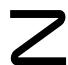
\includegraphics[keepaspectratio]{images/part001_653588be.jpg}}

\begin{enumerate}
\def\labelenumi{\arabic{enumi})}
\setcounter{enumi}{1}
\tightlist
\item
  Let A be a commutative ring. The set of nilpotent elements \(a\) of A is an ideal \(\mathfrak{N}(\mathrm{A})\) of A, called the nilradical of A; it is the intersection of the prime ideals of A (V, §15, No.~1, p.~118, Proposition 2). We have \(\mathfrak{N}(A) \subset \mathfrak{R}(A)\) ; *we have equality if A is an Artinian ring (VIII, p.~173, Corollary 2) or a finitely generated commutative algebra over a commutative field (Comm. Alg., V, §3, n°4, Theorem 3)*. We can certainly have \(\mathfrak{N}(A) \neq \mathfrak{R}(A)\) . This is the case when A is the ring K{[}{[}X{]}{]}, where K is a commutative field: we then have \(\mathfrak{N}(A) = 0\) and \(\mathfrak{R}(A) = AX\) (VIII, p.~154, Example 2).
\end{enumerate}

